\chapter{Metodologia}\label{capitulo2}

Para realizar nossa análise do perfil empreendedor, utilizamos de um questionário composto somente de perguntas objetivas (Consulte o apêndice \ref{Questionario}) divididas em dois grupos: perguntas para analisar do perfil social do aluno \textbf{(Grupo S)} e perguntas para analisar habilidades e conhecimentos relacionados ao perfil empreendedor \textbf{(Grupo E)}. Este questionário foi mapeado em um modelo do Google Forms e então aplicado, por meio da divulgação do link de acesso, às turmas de 1º, 2º e 3º ano dos cursos de Técnico em Informática e Técnico em Química do IFNMG - Campus Montes Claros. O formulário ficou aberto durante duas semanas e foram recolhidas 58 respostas.

Após o recolhimento dos dados, aplicaremos sobre eles ferramentas computacionais para extrair maiores informações. O processo de tratamento e manipulação dos dados será explicado, mas a codificação omitida em sua maioria devido ao foco desse trabalho não serem as ferramentas, mas sim os resultados.

\section{Dados da Pesquisa}
Inicialmente, a própria ferramenta do Google nos fornece algumas informações sobre o perfil social do aluno utilizando da distribuição das respostas por curso, por ano, por gênero, por moradia e por possuir ou não renda pessoal (\ref{fig:quest1-5}).

Ainda utilizando o Google Forms, recolhemos as informações gráficas sobre as distribuições das respostas pertencentes ao grupo E: características do empreendedor (\ref{fig:caract}) e crenças sobre o empreendedorismo (\ref{fig:mv1-2}, \ref{fig:mv3-4} e \ref{fig:mv5}).

\begin{figure}[!h]
    \centering
    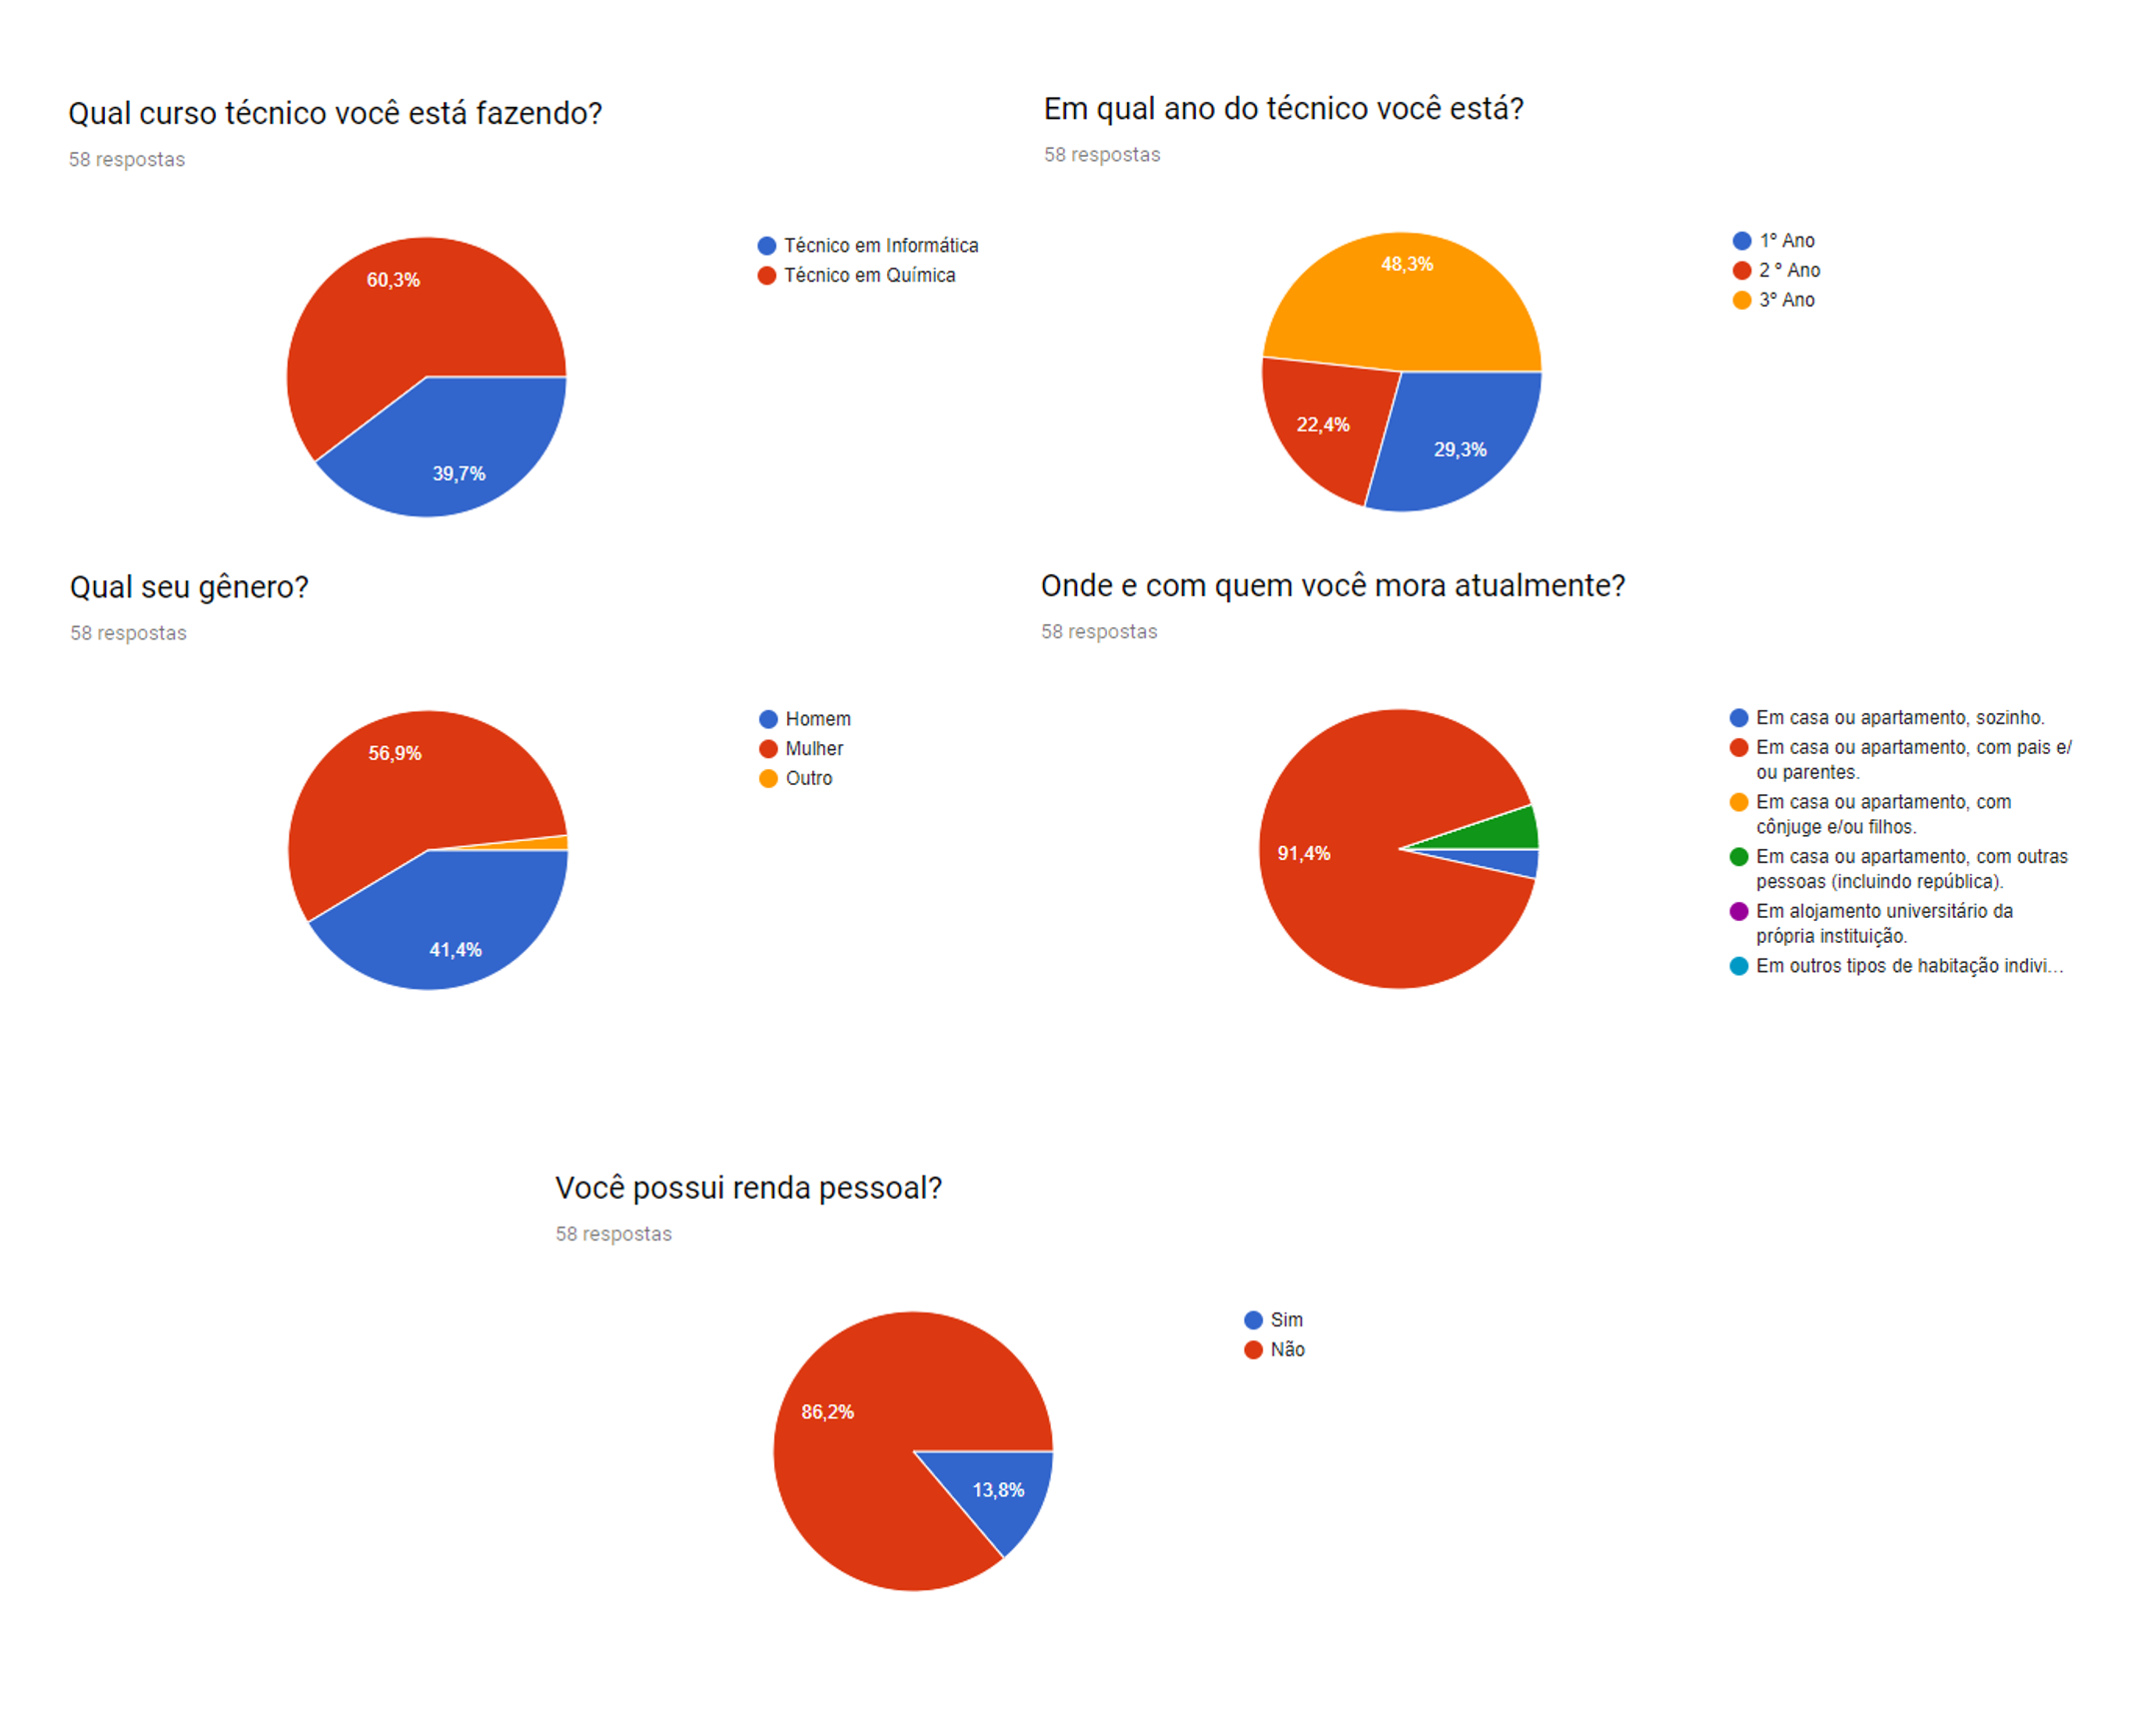
\includegraphics[width=1.0\textwidth]{img/quest1-5.png}
    \caption{Perguntas n$^{\underline{\circ}}$ 1 a 5}
    \label{fig:quest1-5}
\end{figure}

\begin{figure}[H]
    \centering
    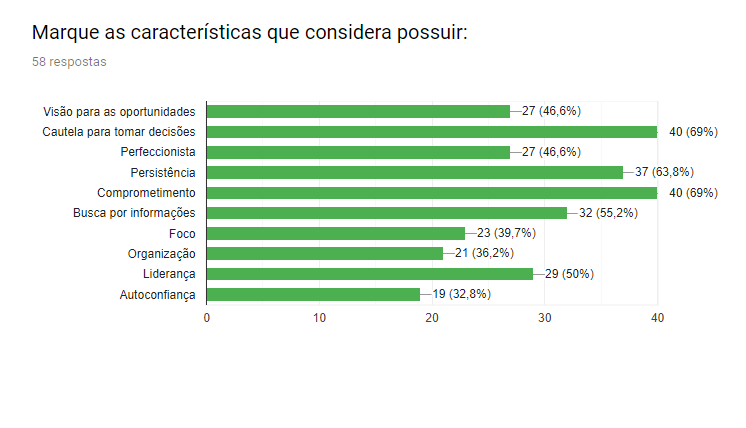
\includegraphics[width=0.9\textwidth]{img/habilidades.PNG}
    \caption{Características que os alunos acreditam possuir.}
    \label{fig:caract}
\end{figure}

\begin{figure}[!h]
    \centering
    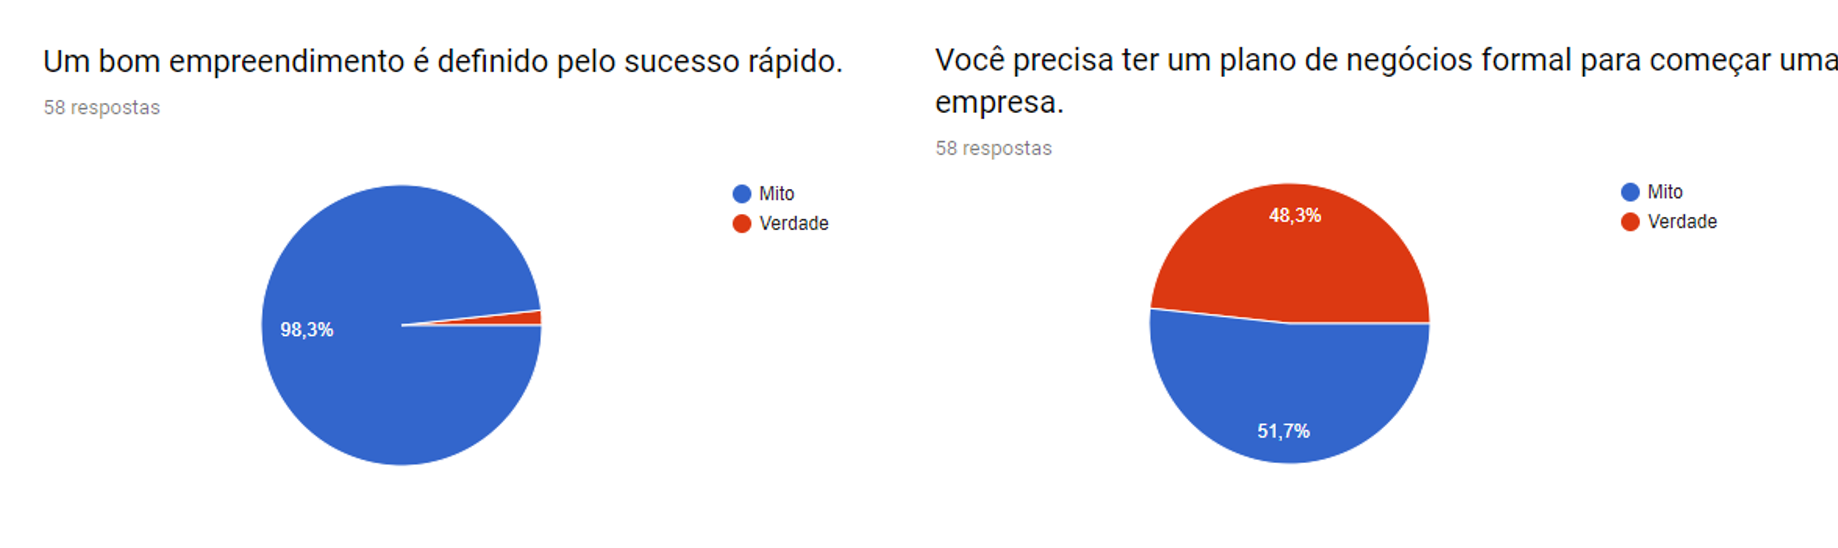
\includegraphics[width=1.0\textwidth]{img/mv1-2.png}
    \caption{Mitos e Verdades (a : Mito) e (b : Mito).}
    \label{fig:mv1-2}
\end{figure}

\begin{figure}[!h]
    \centering
    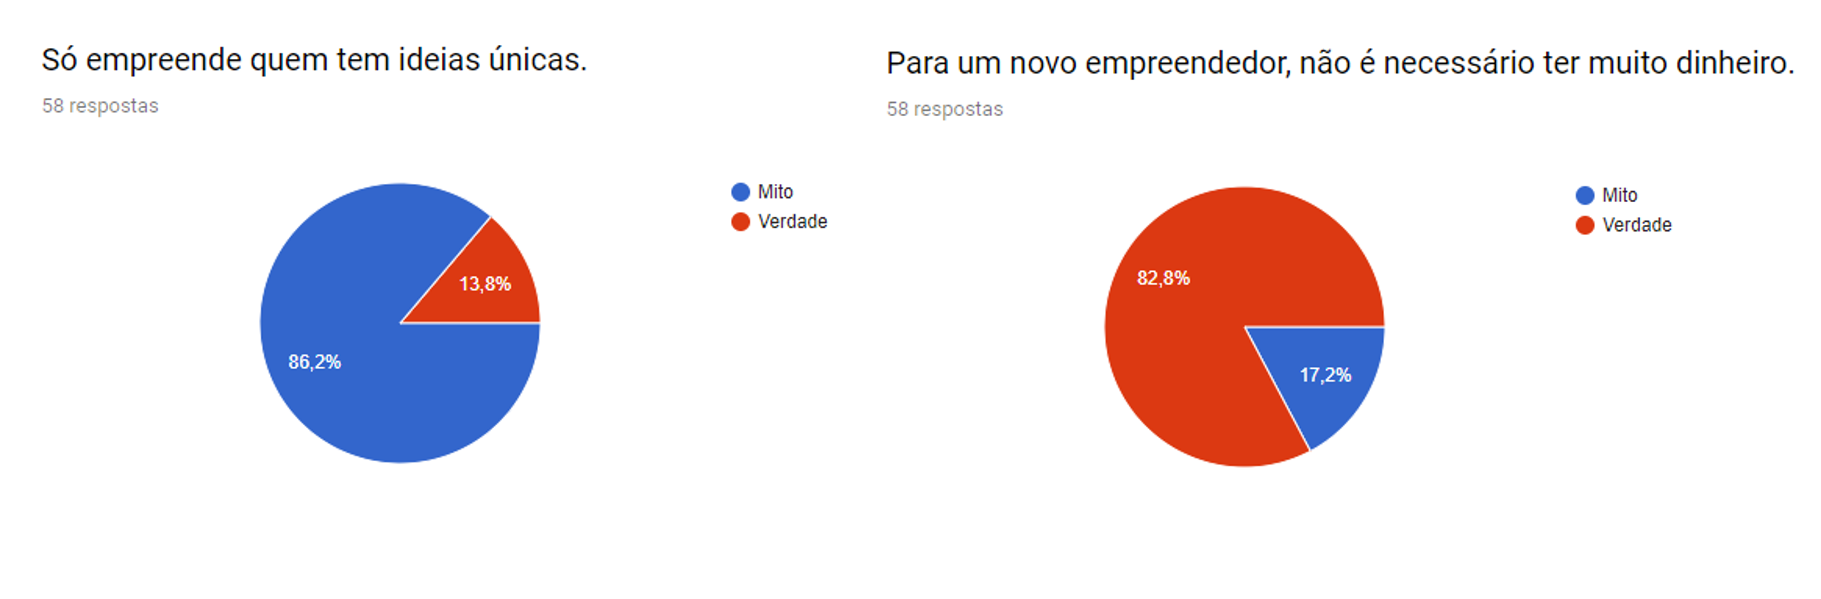
\includegraphics[width=1.0\textwidth]{img/mv3-4.png}
    \caption{ Mitos e Verdades (c : Mito) e (d : Verdade).}
    \label{fig:mv3-4}
\end{figure}

\begin{figure}[!h]
    \centering
    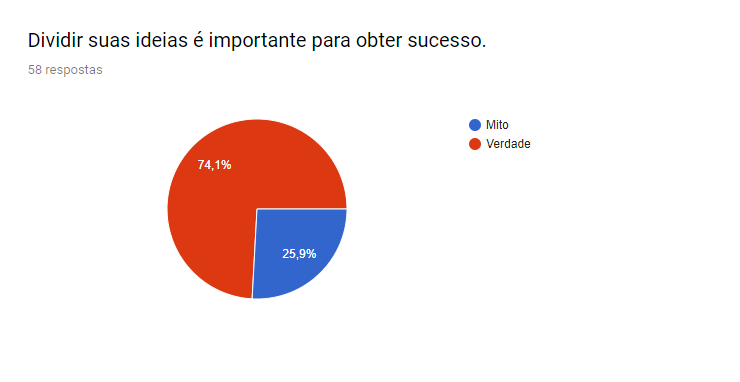
\includegraphics[width=0.7\textwidth]{img/mv5.PNG}
    \caption{Mitos e Verdades (e : Verdade)}
    \label{fig:mv5}
\end{figure}

\section{Análise Exploratória}
De posse dos dados puros da pesquisa, é possível realizar a análise exploratória sobre eles de forma a extrair maiores informações sobre o perfil empreendedor. Faremos essa análise por meio dos subconjuntos de respostas. Por exemplo, podemos extrair as características comuns a empreendedores que os alunos acreditam possuir, restrito somente ao subconjunto de um curso técnico, ou analisar a diferença dessas características entre aqueles alunos que possuem e os não possuem renda pessoal. Sobre as perguntas que dizem respeito aos mitos e verdades, podemos verificar a taxa média de acerto para diversos sub-grupos de nossa pesquisa.

A realização da análise exploratória dos dados foi realizada utilizando a linguagem de programação Python na versão 3.5. Ela oferece diversas facilidades para agrupar, selecionar, alterar, mapear e exibir resultados gráficos dentro de uma base de dados. Além disso, suas ferramentas são  validadas e amplamente utilizadas pela comunidade científica na área de computação.

\subsection{Etapas para a manipulação dos dados}
Inicialmente, os dados da pesquisa foram organizados em uma tabela como mostra a figura \ref{fig:tableB}. Os dados da tabela são convertidos para inteiros, como uma forma de discretizar o espaço de respostas. As respostas discretizadas permitem exibir palavras de frase como conjunto de pontos em gráficos, ou realizar operações como soma das ocorrências das características respondidas. As figuras \ref{fig:tableC1} e \ref{fig:tableC2} mostram a nova configuração da tabela.

\begin{figure}[!h]
    \centering
    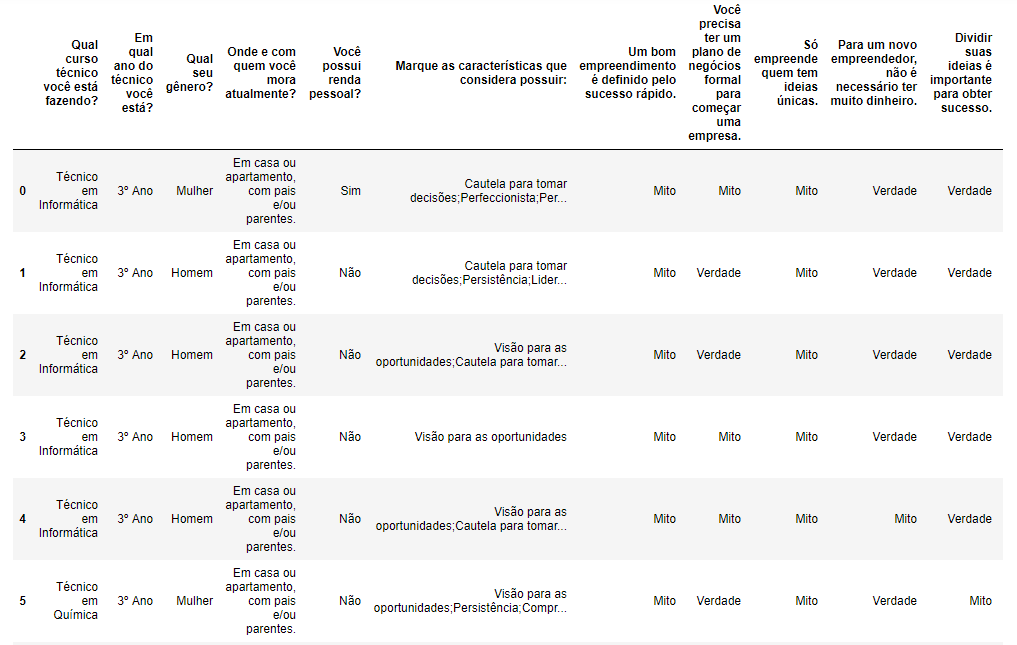
\includegraphics[width=1.0\textwidth]{img/dataFrameBasic.PNG}
    \caption{Primeiras 5 respostas organizadas em tabela.}
    \label{fig:tableB}
\end{figure}

\begin{figure}[!h]
    \centering
    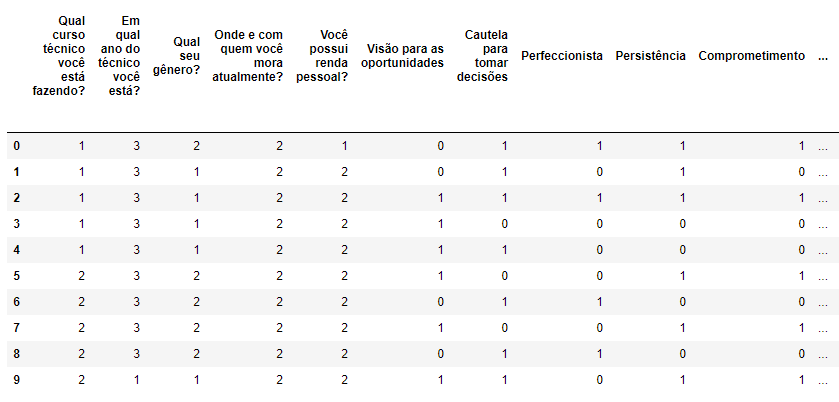
\includegraphics[width=1.0\textwidth]{img/dataFrameConverter1.PNG}
    \caption{Tabela discretizada: Parte 1/2}
    \label{fig:tableC1}
\end{figure}

\begin{figure}[!h]
    \centering
    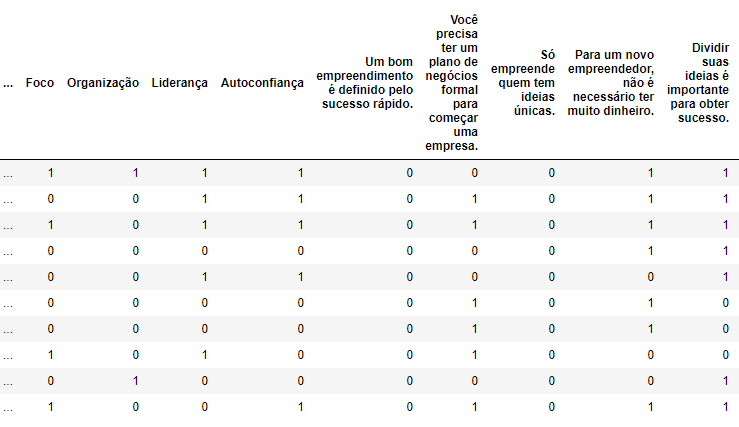
\includegraphics[width=1.0\textwidth]{img/dataFrameConverter2.PNG}
    \caption{Tabela discretizada: Parte 2/2}
    \label{fig:tableC2}
\end{figure}

\subsection{Subconjuntos das Respostas}
Geramos 10 subconjuntos a partir das 58 repostas. Esses subconjuntos não são todos mutuamente exclusivos, mas foram gerados por alguma propriedade importante em nossa análise. Abaixo listamos os conjuntos gerados e suas dimensões.

\begin{itemize}[noitemsep]
    \item Técnico em Informática: 23
    \item Técnico em Informática (1º Ano): 7
    \item Técnico em Informática (2º Ano): 6
    \item Técnico em Informática (3º Ano): 10
    \item Técnico em Química: 35
    \item Técnico em Química (1º Ano): 10
    \item Técnico em Química (2º Ano): 7
    \item Técnico em Química (3º Ano): 18
    \item Possui Renda pessoal: 8
    \item Não Possui Renda pessoal: 50
\end{itemize}

De posse dessas subconjuntos, produzimos as seguintes contagens mostradas nas figuras de  \ref{fig:CaracTecI} até \ref{fig:acertos}

\begin{figure}[!h]
    \centering
    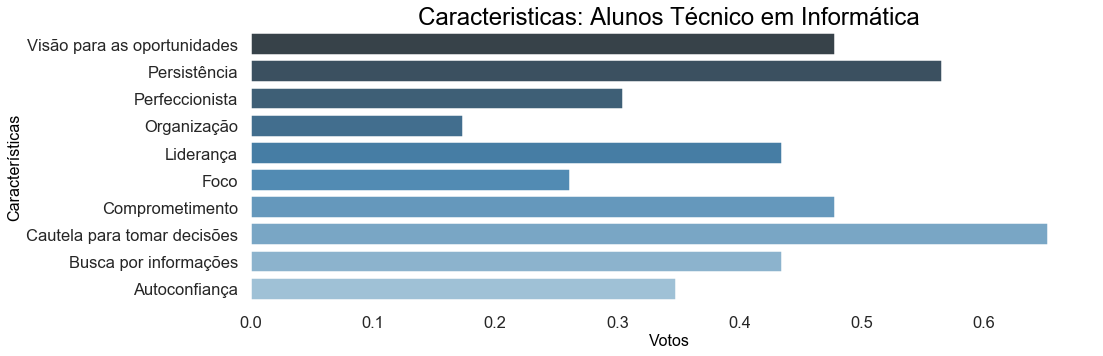
\includegraphics[width=1.0\textwidth]{img/caractTecInf.png}
    \caption{Média: Características Técnico em Informática}
    \label{fig:CaracTecI}
\end{figure}

\begin{figure}[!h]
    \centering
    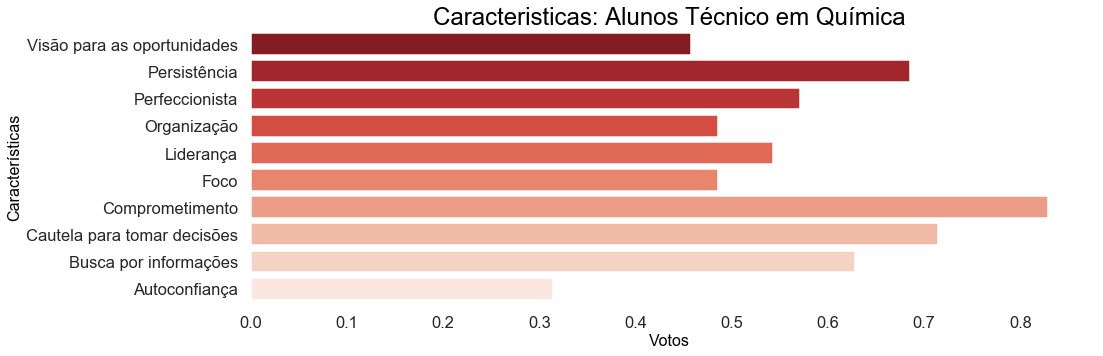
\includegraphics[width=1.0\textwidth]{img/caractTecQui.png}
    \caption{Média: Características Técnico em Química}
    \label{fig:CaracTecQ}
\end{figure}

\begin{figure}[!h]
    \centering
    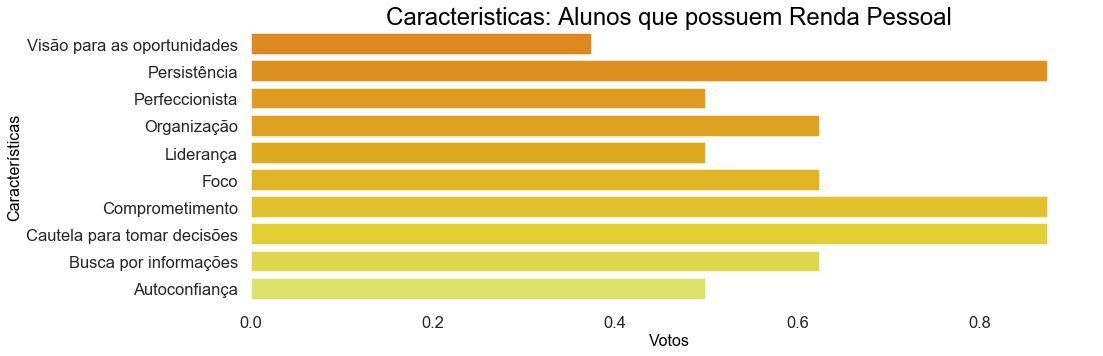
\includegraphics[width=1.0\textwidth]{img/caractRenda.png}
    \caption{Média: Possui Renda Pessoal}
    \label{fig:pRenda}
\end{figure}

\begin{figure}[!h]
    \centering
    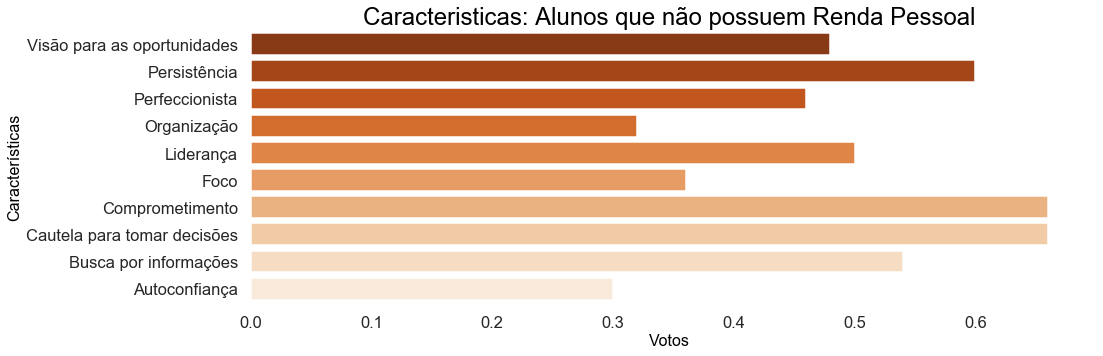
\includegraphics[width=1.0\textwidth]{img/caractNRenda.png}
    \caption{Média: Não Possui Renda Pessoal}
    \label{fig:npRenda}
\end{figure}

\begin{figure}[!h]
    \centering
    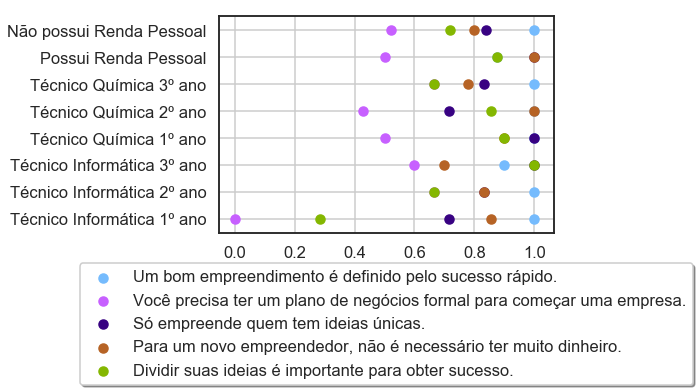
\includegraphics[width=1.0\textwidth]{img/respMV.png}
    \caption{Porcentagem de acertos}
    \label{fig:acertos}
\end{figure}